\documentclass[12pt, titlepage]{report}
\usepackage{consumer_resource_final}
\graphicspath{{./figures/}}

\begin{document}

\section{Building the model numerically}
We want to be able to build feasible models numerically, \ie we would like to generate a set of constant numbers $\{
l_\nu, m_\nu, R^*_\nu, S^*_j, \gamma_{j\nu}, \alpha_{\nu j}, \sigma_{j\nu}, \tau_{j\nu}\}$ such that the equilibria equations Eqs.\eqref{eq : equilibrium resources and species} are fulfilled.


\subsection{Algorithmic procedure}
We hereby detail the procedure used to numerically build feasible systems. It goes like this:
\begin{enumerate}
  \item We first draw randomly $R^*_\nu$
  and $S^*_i$ as a uniform distribution of mean equal to the corresponding metaparameter, \ie :
  \begin{equation}
    \sum_\nu R^*_\nu = N_R R_0 \text{ and } \sum_i S^*_i = N_S S_0.
  \end{equation}
  \item The efficiency matrix $\sigma_{i\nu}$ is then drawn similarly, on a uniform distribution such that $\sigma_0$ is the average of the matrix :
  \begin{equation}
    \sum_{i,\nu} \sigma_{i\nu} = N_S N_R \sigma_0.
  \end{equation}
  \item We build gamma using the desired \textit{food matrix} $F$. $F$ is a binary matrix given by the user (in the \code{configuration.in} file) and is defined as the adjacency matrix of the consumption network (\ie it tells which species eats which resource). We then build $\gamma$ with the same network structure as $F$ (\ie both matrices have the same zero elements). The consumption rates are then randomly drawn from a uniform distribution and $\gamma$ is rescaled such that $\gamma_0$ represents the average consumption rate of the system :
  \begin{equation}
    \sum_{i,\nu} \gamma_{i\nu} = N_S N_R \gamma_0.
  \end{equation}
  \item We then need to build $\alpha_{\nu i}$. This is the tricky part of the algorithm because there are constraints on $\alpha$, for instance energy conservation/dissipation Eq.\eqref{eq : dissipation constraint}. The general strategy is to assume that the metaparameters are chosen in a way that those constraints will practically always be satisfied (see above). We can then build $\alpha$ from a random uniform distribution such that:
  \begin{equation}
    \sum_{i,\nu} \alpha_{\nu i} = N_S N_R \alpha_0.
  \end{equation}
  If for some reason the algorithm fails to build a feasible system this way after a given number of attempts, the $\alpha_{\nu i}$ are drawn by the algorithm and the initial $\alpha_0$ is rescaled accordingly.
  \item We build $\tau_{\nu i}$. It usually is equal to $\alpha_{\nu i}$ or 0.
  \item With all of these parameters drawn, we can solve Eq.\eqref{eq : equilibrium species} for the species death rate $d_i$ (with the caveat that $d_i > 0$, this is one of the constraints on $\tau$ and hence $\alpha$).
  \item Finally, we solve Eq.\eqref{eq : equilibrium resources} for $l_\nu$ and $m_\nu$ imposing the constraint $l_\nu, m_\nu > 0$. In practice this means one of them is drawn randomly (in the code, $l_\nu$ comes from an exponential distribution) with constraints (in the code the minimum value of $l_\nu$) such that both $l_\nu$ and $m_\nu$ are positive.
\end{enumerate}

\section{Conditions on the model parameters}
Although many studies focus on the study of systems described by random $\gamma, \sigma$ or $\alpha$ matrices [\textbf{insert ref}], we will focus on systems that respect physical or biological constraints given below. Those systems are called \textit{feasible}.
\subsection{Energy conservation/dissipation}
The first condition we will impose on our systems is that they do not create new matter.

Remember that in our model, the total amount of biomass given to the species $i$ by the resources is $\sum_\nu \gamma_{i\nu}R_\nu S_i$.
However species $i$ will not allocate all of this biomass to growth. As seen in Eq.\eqref{eq : differential eq for species}, only a fraction $\sigma_{i\nu}$ will be used in this purpose. This means species $i$ disposes of $\sum_\nu(1-\sigma_{i\mu})\gamma_{i\mu}R_\mu S_i$ biomass to complete other processes.
We know that one of these is producing byproducts (\ie the syntrophic interaction) at a total rate $\sum_\nu \alpha_{\nu i} S_i$. Because this biomass is produced in the cell, it has to come from the biomass the cell disposes of, which naturally leads to the condition\footnote{Note that the condition is a bit relaxed here. Biomass cannot be created at equilibrium. However we allow some transient regimes where this momentarily can occur, \eg after a big shock inflicted to the system.}:
  \begin{equation}
  \sum_{\nu} \left(1-\sigma_{i\nu}\right)\gamma_{i\nu}R^*_\nu \geq \sum_\nu \alpha_{\nu i} \label{eq : dissipation constraint}
\end{equation}
The above equation will be referred to as the \textit{conservation of biomass constraint}.

The idea is to find metaparameters such that this constraint is automatically satisfied (which eases building the system numerically). This is easily done by finding the minimum of the LHS and maximum of RHS of Eq.\eqref{eq : dissipation constraint}. Indeed :
\begin{equation}
  \sum_{\nu} \left(1-\sigma_{i\nu}\right)\gamma_{i\nu}R^*_\nu \geq (1-\maxd{\sigma})\mind{\gamma}\mind{R^*},
\end{equation}
where \ $\mind{ }$ \ denotes the minimum value of the random variable and \ $\maxd{ }$ \ its maximum value. On the other hand,
\begin{equation}
  \sum_\nu \alpha_{\nu i} \leq \maxd{\alpha} N_R.
\end{equation}
This means that if we take metaparameters such that
\begin{equation}
  \maxd{\alpha} N_R < (1-\maxd{\sigma})\mind{\gamma}\mind{R^*}, \label{eq : min and max energy constraint}
\end{equation}
then Eq.\eqref{eq : dissipation constraint} is automatically followed.

Because of the way we choose our variables we have for every random variable in the problem,
\begin{equation}
\mind{X} = (1-\epsilon)\mean{X} \text{ and }\maxd{X} = (1+\epsilon)\mean{X}
\end{equation}
where \ $\mean{X}$ \ denotes the mean of $X$. This means Eq.\eqref{eq : min and max energy constraint} is equivalent to, in terms of metaparameters:
\begin{equation}
  \alpha_0 < \frac{\left(1-\epsilon\right)^2}{1+\epsilon}\left(1-\left(1+\epsilon\right)\sigma_0\right)\frac{\gamma_0 R_0}{N_R}.
\end{equation}
In the $\epsilon \ll 1$ limit, this is equivalent to:
\begin{equation}
  \alpha_0 < \left(1-3\epsilon\right)\left(1-(1+\epsilon)\sigma_0\right)\frac{\gamma_0 R_0}{N_R}.
\end{equation}
% \begin{equation}
%   \sum_{\nu} \left(1-\sigma_{i\nu}\right)\gamma_{i\nu}R^*_\nu \geq \min_\nu\left(\left(1-\sigma_{i\nu}\right)R^*_\nu\right) \sum_\nu \gamma_{i\nu} \geq \left(1-\max_\nu\left(\sigma_{i\nu}\right)\right)\min_\nu\left(R^*_\nu\right)N_R \gamma_0.
% \end{equation}
% Now, the way we draw the $\sigma_{i\nu}$ numerically is effectively by drawing elements of a uniform distribution of mean $\sigma_0$, i.e.
% \begin{equation}
%   \sigma_{i\nu} \approx \text{Unif}(0, 2\sigma_0).
% \end{equation}
% It is quite easy to estimate $\max_\nu(\sigma_{i\nu})$, indeed we can easily show that :
% \begin{equation}
%   E\left[\max_\nu\left(\sigma_{i\nu}\right)\right] = 2 \sigma_0 \frac{N_R}{N_R+1}.
% \end{equation}
% This has a standard deviation
% \begin{equation}
%   \tilde{\sigma} = \frac{2 \sigma_0}{N_R+1}\sqrt{\frac{N_R}{N_R+2}}.
% \end{equation}
% Similarly one can show that if
% \begin{equation}
%   R^*_\nu \approx \text{Unif}(0,2R_0),
% \end{equation}
% then
% \begin{equation}
%   E\left[\min_\nu \left(R^*_\nu\right)\right]  = \frac{2R_0}{N_R+1}.
% \end{equation}
% Then we can estimate
% \begin{equation}
%   \left(1-\max_\nu\left(\sigma_{i\nu}\right)\right)\min_\nu\left(R^*_\nu\right)N_R \gamma_0 \approx 2R_0\gamma_0\left(1-2\sigma_0 \frac{N_R}{N_R+1}\right)\frac{N_R}{N_R+1}
% \end{equation}
% We now find an upperbound for the RHS of Eq.\eqref{eq : dissipation constraint} :
% \begin{equation}
%   \sum_\nu \alpha_{\nu i}  \leq \sum_\nu \max_\nu\left(\alpha_{\nu i}\right) \approx 2\alpha_0 \frac{N_R}{N_R+1} N_R.
% \end{equation}
% This means that if we pick metaparameters verifying :
% \begin{equation}
%   R_0 \gamma_0 \left(1-2\sigma_0\frac{N_R}{N_R+1}\right) \gg \alpha_0 N_R.
% \end{equation}
% In the $N_R \gg 1$ limit :
% \begin{equation}
%   \frac{\gamma_0}{\alpha_0} \gg \frac{N_R}{R_0(1-2\sigma_0)}.
% \end{equation}
% This condition allows us to pick metaparameters that we know will satisfy the energy constraint most of the time. This is done solely to speed up computation time (energy constraint is checked anyway while building the system).

\subsection{Positivity of the parameters}
Feasability means at least that every physical parameter defined here must be positive. In particular, this implies:
\begin{equation}
  d_i > 0 \implies \sum_\mu \sigma_{i\mu}\gamma_{i\mu}R^*_\mu > \sum_\mu \tau_{\mu i}
\end{equation}
If $\tau_{i\mu} = 0.$ this is trivially satisfied because $\sigma_{i\mu}$, $\gamma_{i\mu}$ and $R^*_\mu$ have all been drawn positive. However if $\tau_{\mu i} = \alpha_{\mu i}$ this is not always the case and we have to get parameters satisfying :
\begin{equation}
  \sum_\mu \sigma_{i \mu} \gamma_{i\mu}R^*_\mu > \sum_{\mu} \alpha_{\mu i}\text{ }\forall i.
\end{equation}
We can try to estimate the value of some metaparameters that would satisfy this.
We have :
\begin{equation}
  \sum_\mu \sigma_{i\mu} \gamma_{i\mu} R^*_\mu \geq \mind{\sigma}\mind{\gamma}\mind{R^*}.
\end{equation}
Using this boundary and Eq.\eqref{eq : min and max energy constraint}, we know that $d_i>0$ if
\begin{equation}
  \maxd{\alpha}N_R \leq \mind{\sigma} \mind{\gamma}\mind{R^*},
\end{equation}
\ie
\begin{equation}
  \alpha_0 < \frac{\left(1-\epsilon\right)^3}{1+\epsilon} \frac{\sigma_0 \gamma_0 R_0}{N_R},
\end{equation}
or in the $\epsilon \ll 1$ limit :
\begin{equation}
  \alpha_0 < \left(1-4\epsilon\right)\frac{\sigma_0 \gamma_0 R_0}{N_R}.
\end{equation}
Similarly we must have a positive death rate for the resources, \ie:
\begin{equation}
  m_\nu = \frac{l_\nu-\sum_j \gamma_{j\nu} R^*_\nu S^*_j+\sum_j \alpha_{\nu j} S^*_j}{R^*_\nu} > 0. \label{eq : positive m_nu}
\end{equation}
This means we have to impose parameters that verify:
\begin{equation}
  l_\nu + \sum_j \alpha_{\nu j}S^*_j > \sum_j \gamma_{j \nu}R^*_\nu S^*_j.
\end{equation}
We can do a reasoning similar to before, \ie find a lower boundary for the LHS and an upper boundary for the RHS.
We have
\begin{equation}
  l_\nu + \sum_{j} \alpha_{\nu j} S^*_j \geq \mind{l} + \mind{\alpha} \mind{S^*}
\end{equation}
and
\begin{equation}
  \sum_j \gamma_{j\nu}R^*_\nu S^*_j \leq N_S \maxd{\gamma}\maxd{R^*}\maxd{S^*}.
\end{equation}
Hence if we get parameters satisfying
\begin{equation}
  \mind{l}+\mind{\alpha}\mind{S^*} > N_S \maxd{\gamma}\maxd{R^*}\maxd{S^*},
\end{equation}
then Eq.\eqref{eq : positive m_nu} will be immediately satisfied. In terms of metaparameters this is equivalent to:
\begin{equation}
  \alpha_0 > \frac{N_S \gamma_0 R_0 S_0 (1+\epsilon)^3-l_0 (1-\epsilon)}{S_0 (1-\epsilon)^2}.\label{eq : alpha lowerbound 0}
\end{equation}
In the $\epsilon \ll 1$ limit this is equivalent to:
\begin{equation}
  \alpha_0 > \left(1+5\epsilon\right)N_S \gamma_0 R_0 - \left(1+\epsilon\right)\frac{l_0}{S_0}.
\end{equation}
(Interesting, if $l_0/S_0$ is large enough, \ie "there is enough food for everyone" then this condition is irrelevant).
% Indeed,
% \begin{equation}
%   \sum_\mu \alpha_{\mu i} \leq \sum_\mu \max_\mu \left(\alpha_{\mu i}\right) \approx 2\alpha_0 \frac{N_R}{N_R+1} N_R \text{
%     (see above).
%   }
% \end{equation}
% Similarly,
% \begin{equation}
%   \sum_{\mu} \sigma_{i\mu}\gamma_{i\mu}R^*_\mu \geq \min_\mu\left(\sigma_{i\mu}R^*_\mu\right)\sum_\mu \gamma_{i\mu} \geq \min_\mu\left(\sigma_{i\mu}\right)\min_\mu\left(R^*_\mu\right) N_R \gamma_0.
% \end{equation}
% Using the estimations for $\min_\mu\left(\sigma_{i\mu}\right)$ and $\min_\mu\left(R^*_\mu\right)$ :
%  \begin{equation}
%    \min_\mu\left(\sigma_{i\mu}\right) \approx E\left[\min_\mu\left(\sigma_{i\mu}\right)\right] = \frac{2 \sigma_0}{N_R+1}\text{, }\min_\mu\left(R^*_\mu\right) \approx E\left[\min_\mu\left(R^*_\mu \right)\right] = \frac{2 R_0}{N_R+1}
%  \end{equation}
%  This means we have to take :
%  \begin{equation}
%    \frac{\gamma_0}{\alpha_0} \gg \frac{N_R(N_R+1)}{2\sigma_0 R_0}.
%  \end{equation}

\subsection{Combining conditions}
If we combine both upperbounds we get a restriction on the metaparameters:
% \begin{equation}
%   \frac{\gamma_0}{\alpha_0} \gg \max\left(\frac{N_R(N_R+1)}{2\sigma_0 R_0}, \frac{N_R}{R_0(1-2\sigma_0)}\right)
% \end{equation}
% To get an idea on the order of magnitude of the ratio $\gamma_0/\alpha_0$ (\ie our order parameter), if we work with $N_R = 25$, $\sigma_0 = 0.2$, $R_0 = 1$, we have
% \begin{equation}
%   \frac{N_R(N_R+1)}{2\sigma_0 R_0} = 1'625 \text{ and } \frac{N_R}{R_0(1-2\sigma_0)} \approx 42
% \end{equation}
% \ie we will need, if $\gamma_0 \approx 1$
% \begin{equation}
%   \alpha_0 \ll 6.1 \times 10^{-4}.
% \end{equation}
% That means only very small metabolite release (this is indeed what we observe numerically).
\begin{subequations}\label{eq : alpha bounds}
\begin{equation}
\alpha_0 < \min\left(\frac{\left(1-\epsilon\right)^2}{1+\epsilon}\left(1-\left(1+\epsilon\right)\sigma_0\right)\frac{\gamma_0 R_0}{N_R}, \frac{\left(1-\epsilon\right)^3}{1+\epsilon} \frac{\sigma_0 \gamma_0 R_0}{N_R}\right). \label{eq : alpha upperbound}
\end{equation}
We of course also get a restriction on the lowerbound of $\alpha_0$ through Eq.\eqref{eq : alpha lowerbound 0}:
\begin{equation}
  \alpha_0 > \frac{N_S \gamma_0 R_0 S_0 (1+\epsilon)^3-l_0 (1-\epsilon)}{S_0 (1-\epsilon)^2}. \label{eq : alpha lowerbound}
\end{equation}
\end{subequations}
To get an idea on the order of magnitude of $\alpha_0$ (which will be our order parameter if $\gamma_0=1$), we have for $N_R=25$, $\sigma_0 = 0.2$, $R_0 = 1$ and $\epsilon=0.1$ :
\begin{equation}
  \alpha_0 < 5.3 \times 10^{-3}.
\end{equation}
So what we see in Eq.\eqref{eq : alpha upperbound} is that $\alpha_0$ has an upper bound which is dictated either by energy conservation or system feasability. What relations do the metaparameters have to fulfill in these two different regimes?

Suppose that the limiting factor is system feasability. That means:
\begin{empheq}{align}
   \frac{\left(1-\epsilon\right)^3}{1+\epsilon} \frac{\sigma_0 \gamma_0 R_0}{N_R} &\leq \frac{\left(1-\epsilon\right)^2}{1+\epsilon}\left(1-\left(1+\epsilon\right)\sigma_0\right)\frac{\gamma_0 R_0}{N_R} \nonumber \\
  \iff  (1-\epsilon) \sigma_0 &\leq 1-(1+\epsilon)\sigma_0 \nonumber\\
  \iff \sigma_0 &\leq \frac{1}{2}
\end{empheq}
This means if $\sigma_0 \leq \frac{1}{2}$, the limiting factor will be system feasability while if $\sigma_0 \geq \frac{1}{2}$, it will be energy conservation.
\section{Improved feasability conditions}
The previous feasability conditions can be significantly improved.
\subsection{Energy conservation/dissipation}
As stated before, energy conservation is the condition that the biomass you release is not greater than what you have left after you grew:
\begin{equation}
\sum_\nu \left(1-\sigma_{i\nu}\right)\gamma_{i\nu}R^*_\nu \geq \sum_\nu \alpha_{\nu i} \ \forall i=1,\dots, N_S \label{eq : feasability energy conservation}
\end{equation}
We use (neglecting the variances of every quantity involved):
\begin{equation}
\sum_\nu \alpha_{\nu i} \approx k_i^\alpha \alpha_0
\end{equation}
where $k_i^\alpha$ is the degree of the $i$-th column of the alpha matrix.
Similarly,
\begin{equation}
\sum_\nu \left(1-\sigma_{i\nu}\right)\gamma_{i\nu} R^*_\nu \approx (1-\sigma_0)R_0\sum_{\nu}\gamma_{i\nu} \approx k_i^\gamma(1-\sigma_0)R_0\gamma_0,
\end{equation}
where $k_i^\gamma$ is the degree of the $i-$th row of the $\gamma$ matrix.
Then energy conservation Eq.\eqref{eq : feasability energy conservation} is equivalent to
\begin{equation}
k_i^\alpha \alpha_0 \lessapprox k_i^\gamma (1-\sigma_0)R_0\gamma_0 \ \forall i=1,...,N_S
\end{equation}
Since $k_i^\gamma > 0 $ (it is the number of resources species $i$ eats), we have:
\begin{equation}
\frac{k_i^\alpha}{k_i^\gamma} \alpha_0 \lessapprox (1-\sigma_0)R_0\gamma_0 \ \forall i=1,...,N_S
\end{equation}
This is fulfilled if :
\begin{equation}
\boxed{
\max_i\left\{\frac{k_i^\alpha}{k_i^\gamma}\right\} \alpha_0 \lessapprox (1-\sigma_0)R_0 \gamma_0
}
\end{equation}
What this basically says is that systems where the ratio $\frac{\# \text{resources released to}}{\# \text{resources consumed}}$ is small for each species allow for a larger individual syntrophy interaction (which is very intuitive).
\subsection{Positivity of the parameters}
As said before, the death rates have to be positive:
\begin{equation}
\sum_\mu \sigma_{i\mu}\gamma_{i\mu}R^*_\mu > \sum_\mu \tau_{\mu i}
\end{equation}
Using a similar reasoning :
\begin{equation}
\boxed{
\max_i\left\{\frac{k_i^\alpha}{k_i^\gamma}\right\} \alpha_0 \lessapprox \sigma_0R_0 \gamma_0
}
\end{equation}
Also for $m_\nu$ to be positive we need:
\begin{equation}
l_\nu + \sum_j \alpha_{\nu j} S^*_j > \sum_j \gamma_{j\nu}R^*_\nu S^*_j \ \forall \nu=1,\dots,N_R
\end{equation}
Which is equivalent to
\begin{equation}
l_0 + k_\nu^\alpha \alpha_0 S_0 \gtrapprox k_\nu^\gamma \gamma_0 R_0 S_0 \ \forall \nu
\end{equation}
Since $k_\nu^\gamma>0$ (every resource is at least consumed by one species), the $N_R$ equations above can be rewritten as:
\begin{equation}
\boxed{
\min_\nu\left\{\frac{l_0}{k_\nu^\gamma S_0} + \frac{k_\nu^\alpha}{k_\nu^\gamma}\alpha_0\right\} \gtrapprox \gamma_0 R_0
}
\end{equation}
This says that systems where the ratio $\frac{\#\text{number of species that release to me}}{\#\text{number of species that consume me}}$ is large for every resource are more feasible. The strategy should be then to have $\gamma$'s that have large $k^\gamma_\nu$ (\ie resources are consumed by many species) and large $k_i^\gamma$ (\ie species consume a lot of species), and the other way around for $\alpha$ (not sure about this for the last one).

\section{Effective system}
Models which involve the dynamics of species only are in general better known than consumers-resources models [\textbf{insert reference}]. In particular, a huge body of literature exists on the study of Lotka-Volterra systems [\textbf{insert reference}]. We may profit from this knowledge by transforming the effect of the resources dynamics into an effective consumers-only system.

This can be done by assuming that the resources reach an equilibrium way faster than the consumers.
Mathematically, that is equivalent to
\begin{equation}
  \frac{dR_\mu}{dt} \approx 0, \\ \forall \mu.
\end{equation}
Using Eq.\eqref{eq : differential eq for resources}, we get an explicit value for the resources:
\begin{equation}
  R_\mu \approx \frac{l_\mu+\sum_j \alpha_{\mu j}S_j}{m_\mu + \sum_k \gamma_{k\mu}S_k}.
\end{equation}
This expression can be used in Eq.\eqref{eq : differential eq for species} to get an effective system which describes the dynamics of the $N_S$ consumers :
\begin{equation}
  \frac{dS_i}{dt} = \left(\sum_\nu \left(\frac{\sigma_{i\nu}\gamma_{i\nu}l_\nu}{m_\nu+\sum_k \gamma_{k\nu}S_k} - \tau_{\nu i}\right) -d_i + \sum_{\nu j} \frac{\sigma_{i\nu}\gamma_{i\nu}\alpha_{\nu j}}{m_\nu+\sum_{k}\gamma_{k\nu}S_k}S_j \right) S_i.
\end{equation}
This can be rewritten in a more compact way:
\begin{equation}
  \frac{dS_i}{dt} = p_i(S) S_i + \sum_j M_{ij}(S)S_i S_j \label{eq : effective equations of evolution}
\end{equation}
with
\begin{equation}
    p_i(S) = -\left(d_i+\sum_{\nu}\tau_{\nu i}\right) + \sum_\nu \frac{\sigma_{i\nu}\gamma_{i\nu}l_\nu}{m_\nu+\sum_k \gamma_{k\nu}S_k}\text{ and } M_{ij}(S)=\sum_{\nu}\frac{\sigma_{i\nu}\gamma_{i\nu}\alpha_{\nu j}}{m_\nu+\sum_{k}\gamma_{k\nu}S_k}.
\end{equation}
If we assume the species $S_k$ are not too far away from their equilibrium values\footnote{Note that this is very rarely true, especially in the context of the study of structural stability, where entire species sometimes die out.}, \ie
\begin{equation}
S_k \approx S^*_k \ \forall k,
\end{equation}
then using Eq.\eqref{eq : positive m_nu} we can simplify $p_i$. Indeed,
\begin{equation}
m_\nu + \sum_k \gamma_{k\nu} S_k \approx m_\nu + \sum_k \gamma_{k\nu}S^*_k = \frac{l_\nu + \sum_k \alpha_{\nu k}S^*_k}{R^*_\nu} \label{eq : equality fluxes resource}
\end{equation}
Hence, the explicit dynamical dependence on $S$ can be removed from $p_i$ and $M_{ij}$:
\begin{equation}
p_i(S) \approx p_i \equiv - \left(d_i + \sum_\nu \tau_{\nu i}\right) + \sum_\nu \frac{\sigma_{i\nu}\gamma_{i\nu}l_\nu R^*_\nu}{l_\nu + \sum_k \alpha_{\nu k}S^*_k},
\end{equation} and
\begin{equation}
M_{ij}(S) \approx M_{ij} \equiv \sum_\nu \frac{\sigma_{i\nu} \gamma_{i\nu} R^*_\nu \alpha_{\nu j}}{l_\nu + \sum_k{\alpha_{\nu k} S^*_k}}.
\end{equation}
\subsection{Perturbation analysis}
We study a system that we put close to an equilibrium $S^*$, \ie
\begin{equation}
S=S^*+\Delta S, \\ \text{with } \Delta S \ll 1.
\end{equation}
Written this way, the effective equations of motion Eq.\eqref{eq : effective equations of evolution} are equivalent to:
\begin{equation}
\frac{d\Delta S_i}{dt} = p_i(S^*+\Delta S)\left(S^*_i + \Delta S_i\right)+\sum_j M_{ij}(S^*+\Delta S)\left(S^*_i +\Delta S_i\right)\left(S^*_j +\Delta S_j\right).
\end{equation}
Since the deviations from equilibrium $\Delta S_i \ll 1$, we can forget the terms in higher power than quadratic:
\begin{equation}
\frac{d\Delta S_i}{dt} = \tilde{p}_i \Delta S_i + \sum_j E_{ij} \Delta S_j + \bigO(\Delta S^2),\label{eq : effective equ evol at O(D2)}
\end{equation}
with
\begin{equation}
\tilde{p}_i \equiv p_i(S^*) + \sum_k M_{ik}(S^*)S_k^*, \label{eq : tilde p effective system}
\end{equation}
and
\begin{equation}
E_{ij} \equiv \left(\partiald{p_i}{S_j}\evaluatedat{S^*}+M_{ij}(S^*)+\sum_k \partiald{M_{ik}}{S_j}\evaluatedat{S^*}S^*_k\right)S^*_i.
\end{equation}
After some computations, we can get $\tilde{p}_i$ and $E_{ij}$ in terms of the initial parameters. Indeed,
\begin{equation}
p_i(S^*)= -\left(d_i + \sum_\nu \tau_{\nu i}\right) + \sum_\nu \frac{\sigma_{i\nu}\gamma_{i\nu}l_\nu}{m_\nu + \sum_k \gamma_{k\nu}S^*_k}
\end{equation}
and
\begin{equation}
M_{ik}(S^*) = \sum_\nu \frac{\sigma_{i\nu}\gamma_{i\nu}\alpha_{\nu j}}{m_\nu + \sum_k \gamma_{k\nu}S^*_k}.
\end{equation}
Hence, using Eq.\eqref{eq : tilde p effective system} :
\begin{equation}
\tilde{p}_i = - \left(d_i + \sum_\nu \tau_{\nu i}\right) + \sum_\nu \frac{\sigma_{i\nu}\gamma_{i\nu}}{m_\nu + \sum_k \gamma_{k\nu}S^*_k}\left(l_\nu+\sum_{j}\alpha_{\nu j} S^*_j\right).
\end{equation}
This can be simplified using Eq.\eqref{eq : equality fluxes resource} and Eq.\eqref{eq : equilibrium species} :
\begin{equation}
\tilde{p}_i=-d_i +\sum_\nu \sigma_{i\nu}\gamma_{i\nu}R^*_\nu = \sum_\nu \tau_{\nu i}.
\end{equation}
With a similar computation, one finds
\begin{equation}
E_{ij}=\sum_\nu \frac{\sigma_{i\nu}\gamma_{i\nu}S^*_i}{m_\nu+\sum_k \gamma_{k\nu}S^*_k} \left(\alpha_{\nu j}-\gamma_{j\nu}R^*_\nu\right).
\end{equation}
Finally, Eq.\eqref{eq : effective equ evol at O(D2)} can be recast in
\begin{equation}
\frac{d\Delta S_i}{dt} = \sum_j (J_E)_{ij} \Delta S_j,
\end{equation}
where the effective $N_S\times N_S$ jacobian matrix $J_E$ is defined by:
\begin{equation}
(J_E)_{ij}=\sum_\nu \left[\frac{\sigma_{i\nu}\gamma_{i\nu}S^*_i}{m_\nu+\sum_k \gamma_{k\nu}S^*_k} \left(\alpha_{\nu j}-\gamma_{j\nu}R^*_\nu\right)+\tau_{\nu i}\delta_{ij}\right].
\end{equation}
We see that we without surprise we find again the $\Beta, \Gamma $ and $\Delta$ matrices coming from the jacobian at equilibrium :
\begin{equation}
\left(J_E\right)_{ij}=\sum_\nu \left[\frac{\Beta_{i\nu}\Gamma_{\nu j}}{\Delta_\nu}+\tau_{\nu i} \delta_{ij}\right]
\end{equation}

This matrix determines the stability of the equilibrium. Namely if the largest eigenvalue of $J_E$ is positive, the equilibrium is unstable. If it is negative, the equilibrium is stable. If it is zero, the equilibrium is marginal.
\section{Numerical simulations}
\subsection{Testing the algorithm}
\subsection{The effect of sigma non uniform}
\begin{figure}
\includegraphics[width=0.6\linewidth]{figures/eigenvalues_Nest015_Conn01808_sigma_uniform}
\caption{Eigenvalues $\kappa=0.1808$, $\eta=0.15$, $R_0=\gamma_0=0.2$, $\alpha_0=0$, $\sigma_0=0.25$, uniform efficiency matrix (Butler case).}
\includegraphics[width=0.6\linewidth]{figures/eigenvalues_Nest015_Conn01808_sigma_spread}
\caption{Eigenvalues $\kappa=0.1808$, $\eta=0.15$, $R_0=\gamma_0=0.2$, $\alpha_0=0$, $\sigma_0=0.25$, efficiency matrix with a spread. We observed some systems with an eigenvalue larger than zero.}
\end{figure}

\subsection{Time evolution}
\begin{figure}[h!]
\centering
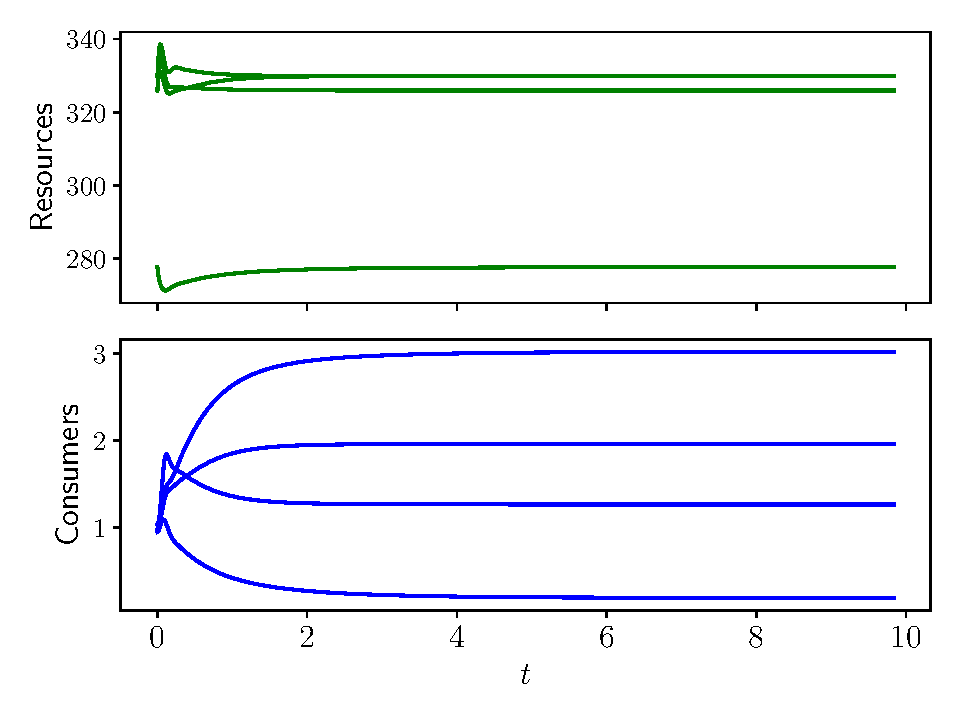
\includegraphics[width=0.6\linewidth]{Typical_time_evolution/Typical_time_evolution_resources_species_high_threshold.pdf}
\caption{Time evolution for high coefficient threshold ($\epsilon_{\text{conv}}=10^{-1}$)}
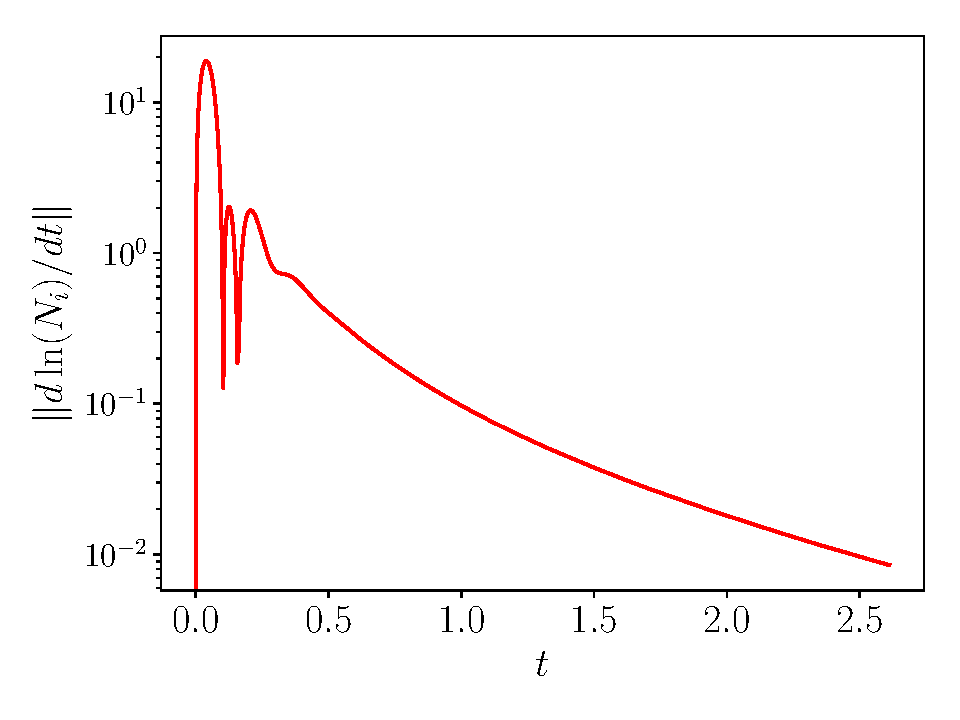
\includegraphics[width=0.6\linewidth]{figures/Typical_time_evolution/Typical_time_evolution_log_derivative_high_threshold.pdf}
\caption{Typical convergence to judge equilibrium, we see the simulation stops at $\epsilon_{\text{conv}}=10^{-1}$}
\end{figure}
\begin{figure}[h!]
\centering
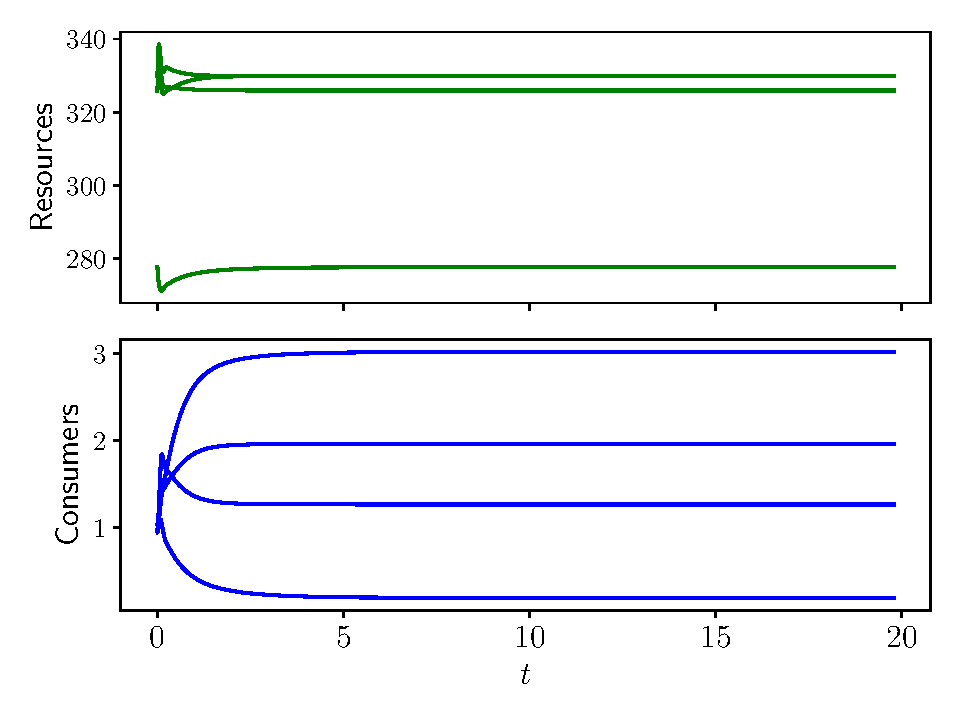
\includegraphics[width=0.6\linewidth]{Typical_time_evolution/Typical_time_evolution_resources_species_low_threshold.pdf}
\caption{Time evolution for low coefficient threshold (more accuracy) ($\epsilon_{\text{conv}}=10^{-5}$)}
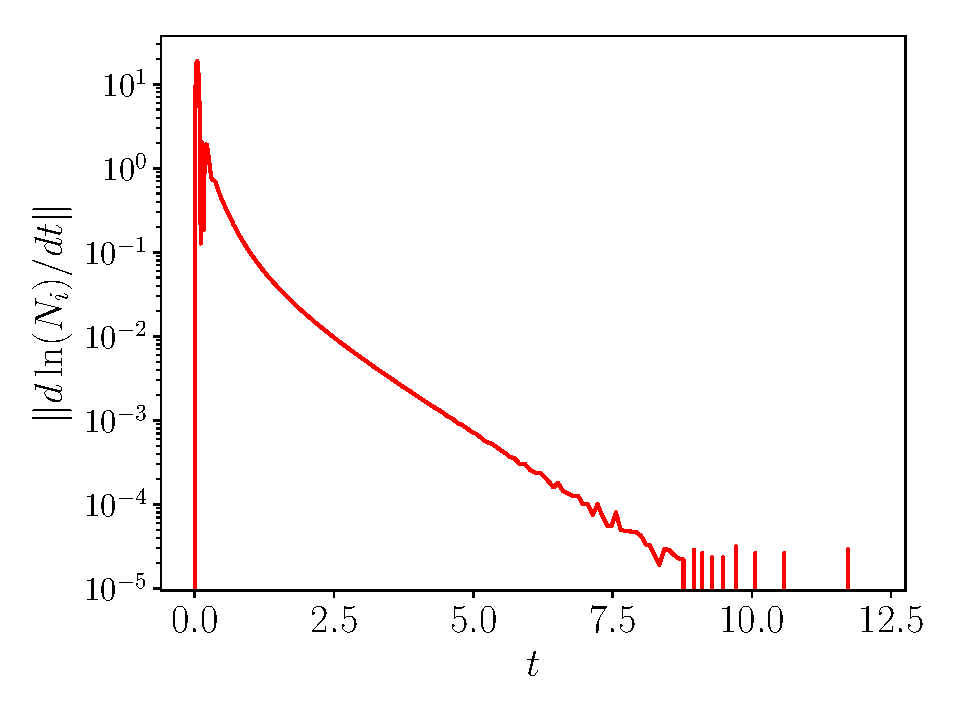
\includegraphics[width=0.6\linewidth]{figures/Typical_time_evolution/Typical_time_evolution_log_derivative_low_threshold.pdf}
\caption{Typical convergence to judge equilibrium, we see the simulation stops at $\epsilon_{\text{conv}}=10^{-5}$}
\end{figure}
\subsection{Allowed parameters : syntrophy range}
\begin{figure}[h!]
\centering
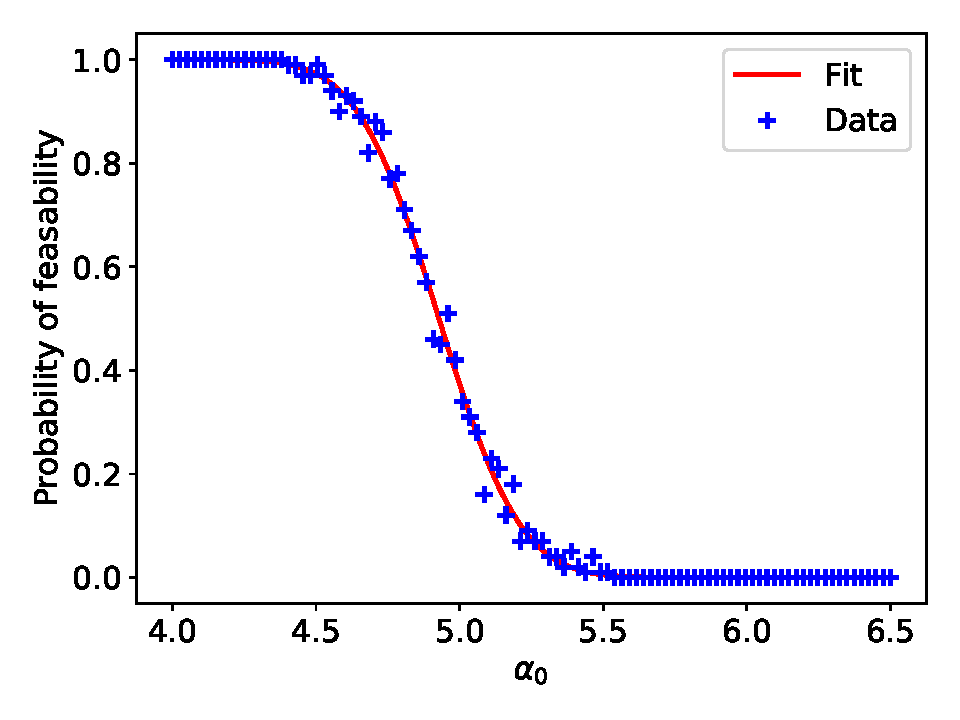
\includegraphics[scale=0.7]{figures/alpha0_probability_of_feasability}
\caption{Typical shape of the probability of feasability for every metaparameter fixed except varying $\alpha_0$. We see that the probability of drawing a feasible system decreases sharply as $\alpha_0$ increases. A typical sigmoidal curve (here an erf function) fits the numerical data quite well.}
\end{figure}

\subsection{Studying the impact of the food network structure}
\subsection{Studying the impact of syntrophy}
We run a bunch of simulations with the following metaparameters. We made sure that these are compatible with the bounds on $\alpha_0$ Eqs.\eqref{eq : alpha bounds}.

% Please add the following required packages to your document preamble:
% \usepackage{graphicx}
\begin{table}[h!]
\centering
\begin{tabular}{c|c|c|c|c|c}
$\gamma_0$ & $\sigma_0$ & $\alpha_0$ & $R_0$ & $S_0$ & $l_0$ \\ \hline
1          & 1          & 0          & 300   & 1     & 11091 \\
         & 0.75       & 0          &       &       &       \\
         &            & 0.5        &       &       &       \\
         & 0.5        & 0          &       &       &       \\
         &            & 0.5        &       &       &       \\
         &            & 1          &       &       &       \\
         & 0.25       & 0          &       &       &       \\
         &            & 0.5        &       &       &       \\
         &            & 1          &       &       &       \\
         &            & 1.5        &       &       &
\end{tabular}
\caption{Metaparameters used for the simulations.} \label{eq : table metaparameters used}
\end{table}
\end{document}
